\chapter{Literature Review}
\section{Brush-less DC motor driving}
\subsection{Brush-less DC motor}
Most UAV platforms spin their propellers using Brushless-DC (BLDC) motors due to their low weight, high top speeds and efficiency. Therefore, it is  imperative to know the basic principles to analyze ESCs. 

A BLDC motor can be 1, 2 or 3-phase. However, the most efficient version at high speeds and the ones used for UAVs is the 3-phase version. Therefore, the BLDC term will refer to 3-phase BLDC motors. Figure \ref{fig:bldcm} shows a simplified diagram with only 4 magnetic poles whereas a typical motor used for UAVs would have 14. Here,the stator includes coils and the rotor has permanent magnets.

\begin{figure}
    \centering
    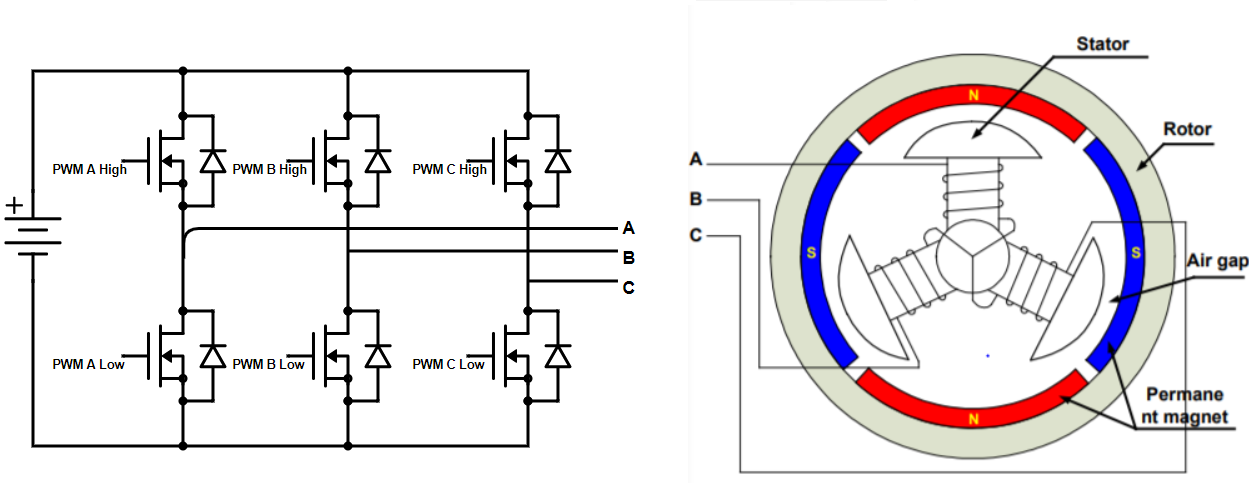
\includegraphics[width=\textwidth]{images/bldcm_diagram.png}
    \caption{\textit{Left} MOSFET bridge driver. \textit{Right} BLDC motor simplified \cite{Zhao_BLDCFundamentals}}
    \label{fig:bldcm}
\end{figure}

\subsection{BLDC motor driving methods}
Two configurations can be used to run BLDC motors as mentioned in \cite{Mogensen_ESC_Motor_Control2016}, both based on Pulse Width Modulation (PWM). These are Trapezoidal and Sinusoidal. They differ in the ideal driving voltage wave-forms to use when driving the motor coils. In both cases, the best performing phase shift between phases is 120\textdegree.  The effective instantaneous voltage in each coil is a fraction of the DC power supply. PWM approximates this fraction by providing a pulsing signal with a corresponding duty cycle (fraction of time the signal is high). 
To generate these PWM signals from a DC power source, power MOSFETs are used in bridge configurations. The specific configuration used for BLDC motors is shown in Figure \ref{fig:bldcm}
\newline

\textit{Trapezoidal:}
Here the ideal driving waveform is a trapezoidal wave. As shown in Figure \ref{fig:foc_trapezoidal_signals} bottom. This method is easier to implement in hardware since a relatively low accuracy in rotor angular position estimation is needed. However, there are significant power loses caused by many spikes in the signal and also because the electrical magnetic field caused by the stator is only instantaneously at the optimal orientation relative to the rotor magnetic field (perpendicular). Here, the duty cycle put through the active phases is constant for the same rotor speed
\newline

\textit{Sinusoidal:}
In this case, the ideal driving waveform is a sinusoid as seen in figure \ref{fig:foc_trapezoidal_signals} top. Note that for the same rotor speed, the duty cycle continuously changes over an electrical period to mimic the ideal sinewave. This is because of the waveform continuously changing and because feedback control \footnote{This is not rotor speed control} is used to maintain the relative orientation rotor-startor magnetic field orientation optimal (90\textdegree). Since the duty cycle is changed more often and depending on the rotor position, this method requires a significantly higher accuracy in rotor angular position estimation.
Higher efficiency is obtained in two fronts:less pulsing implies less spikes and therefore switching power losses; the magnetic fields relative orientation is controlled to be optimal. 

\begin{figure}
    \centering
    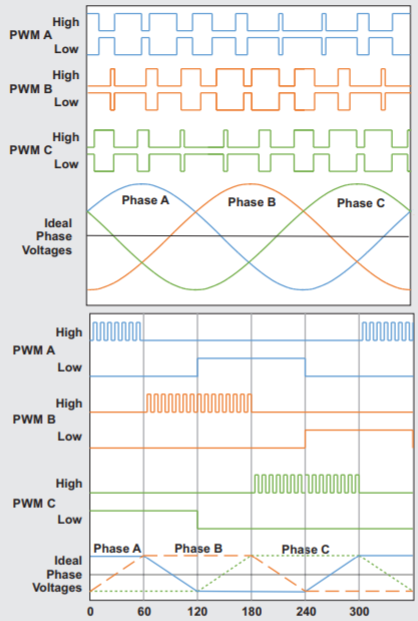
\includegraphics[width=0.5\textwidth]{images/foc_trap_sig.png}
    \caption{PWM Phase signals vs Rotor Position. \textit{Top} Sinusoidal FOC, \textit{Bottom} Trapezoidal. Adapted from \cite{Mogensen_ESC_Motor_Control2016}}
    \label{fig:foc_trapezoidal_signals}
\end{figure}


\section{Electronic Speed Controllers}
\subsection{General structure}
The circuits that run the BLDC motors are commonly known as Electronic Speed Controllers (ESC). However, the majority of current available ones do not perform direct motor speed control. Their core components are a micro-controller, gate drivers, back Electro-motive foce (EMF) measurement resistors and the MOSFETs (shown in Figure \ref{fig:bldcm}). In essence, what they do is receive a throttle signal from a Flight Controller (FC) representing the amplitude of the ideal driving signal (explained in previous subsection, Fig. \ref{fig:foc_trapezoidal_signals}). The diagram in Figure \ref{fig:esc_diag} shows a general electrical architecture of ESCs. Note that gate drivers are simply interface circuits that allow to turn on/off the MOSFETs.
\begin{figure}
    \centering
    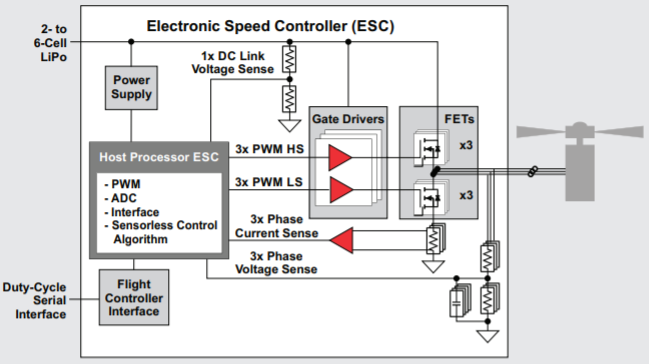
\includegraphics[width=0.8\textwidth]{images/esc_diagram.PNG}
    \caption{ESC general architecture \cite{Mogensen_ESC_Motor_Control2016}}
    \label{fig:esc_diag}
\end{figure}

\subsection{Communications}
ESCs need to communicate with the FC to receive throttle commands and in some cases they also send status messages. Hence, some protocols have been used and other have been developed in the context of UAVs.

\subsubsection{Analog Protocols}
All of these protocols are based on Pulse width modulation given a maximum and a minimum pulse width to be set as maximum and minimum throttle. Hence, these protocols are commonly called RCPWM. Thee different protocols in this category merely differ in the pulse period. Figure \ref{fig:oneshot_dshot} depicts these kind of signals on the top and Table \ref{tab:tab_escs}  shows their transmission parameters.

\begin{figure}
    \centering
    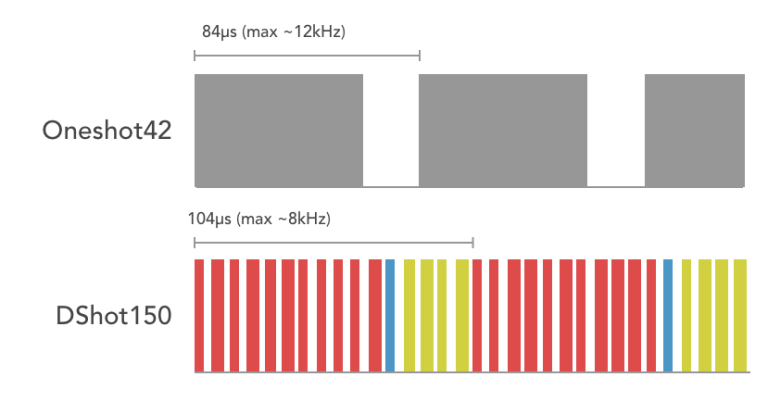
\includegraphics[width=0.8\textwidth]{images/oneshot_dshot.png}
    \caption{Oneshot vs Dshot comparison \cite{BackyardRobotics2018}}
    \label{fig:oneshot_dshot}
\end{figure}

\begin{table}
\begin{center}
 \caption{ESC protocols' speeds}\vspace{1ex}
 \label{tab:tab_escs}
 \begin{tabular}{l|rrr}
 \hline
Protocol & Type & Pulse width range [$\mu s$] & Max Update Rate [kHz] \\ \hline \hline
PWM                 & Analog & 1000 - 2000  & 0.490\\
Oneshot125          & Analog & 125 - 250    & 4\\
Oneshot42           & Analog & 42 - 84      & 12\\
Multishot           & Analog & 5 - 25       & 40\\
Dshot150            & Digital & 106.8        & 9\\
Dshot300            & Digital & 53.4         & 18\\
Dshot600            & Digital & 26.7         & 37\\
Dshot1200           & Digital & 13.4         & 75\\
Bidirectional Dshot & Digital & Dshot values & Dshot values \\
Proshot             & Digital & Dshot values & Dshot values\\
UAVCAN              & Digital & NA           & NA\\
 \end{tabular}
\end{center}
\end{table}


\subsubsection{Digital Protocols}
Even though most of these protocols are widely known as digital, the true purely digital protocol is UAVCAN. The rest define certain specific pulse time durations to high or low. Dshot will be explained thoroughly in particular given that it's the basis of all the other methods but UAVCAN.
\newline
\textit{Dshot: } This method consists of a 16-bit packet streamed continuously. Each bit is encoded as a pulse with one of to widths, depending on the pulse width version. Figure \ref{fig:oneshot_dshot} show a comparison of the Dshot signals with PWM signals and Figure XXXXX shows the information organization in each packet. The packet is divided into three sections as shown in Figure : 
\begin{itemize}
    \item Throttle command: Consists of 11 bits (Decimal values 0 -2047). Commands in the range [0,47] are status request commands whereas values in the range [48,2047] encode a 2000 levels throttle command.
    \item Telemetry request: When this bit is high, telemetry is hight, the ESC is sends a telemetry information packet from the to the FC. Including information such as: Motor Electrical RPM, ESC Temperature, Supply Voltage, Current (Available only in certain ESCs).
    \item Cyclic Redundancy Check (CRC): Used to check for data corruption during transmission.
\end{itemize}



\section{Pixhawk 4 and PX4 architecture}
Flight controllers are the core component of a UAV as they order the ESCs to provide rotor speeds that stabilize and move the aircraft. 

\section{Related Work on ESCs characterization}
